%\chapter{Theory Introduction}  % should probably change this name
%\chapter{Introduction to Theory Background} \footnote
\chapter[Introduction to Theory Background]{Introduction to Theory Background \protect\footnote{Much of the material for this chapter was taken from \cite{HM}.}}
\label{theory}

Any physics analysis must be based on a 
solid understanding of the 
underlying theory and mathematics.  
This chapter's aim is to introduce 
the background for a Z production 
cross section analysis.  

% \cite{HM}  HALZEN AND MARTIN REFERENCE FOOTNOTE

\section{The Standard Model}
\label{theory:SM}

% quarks, leptons, bosons!  HIGGS ha ha
% make separate paragraphs for different types?  or sections?  that's how other people did it

% MAKE TABLE SHOWING WHAT FEELS WHAT FORCE!  or something -- quantum number is more complicated way of showing it.  draw connection in text

% EXPLAIN SQUARE ROOT OF S so do need to get into s.  okay, via s-level diagram

The Standard Model describes the current understanding 
of how fundamental particles interact.  
There are three different types of particles: 
quarks and leptons, 
which make up matter, 
and bosons, which transmit forces.  
Quarks and leptons are collectively called fermions; 
%because they have spin-$\frac{1}{2}$   % HAVE TO EXPLAIN SPIN AND ALL THAT???
two fermions cannot exist in the same state as each other.  
Bosons do not have this constraint; 
many bosons can be in the same state.  
The particles are shown in Figure~\ref{fig:StandardModel}, 
with more detailed information given in 
Table~\ref{TableSMParticles}. 
The first three columns show the first three generations 
of the quarks and leptons, 
while the last column shows the bosons.  
Each fermion generation contains two quarks, 
a neutrino, and a charged lepton.  
In general, the generations get progressively heavier.  
The electron is lighter than the muon, 
which is lighter than the $\tau$.   
The same relation exists between the quark generations; 
the top quark is the heaviest known particle in the Standard Model.  % CHECK!!!!!
Normal, everyday matter is made up solely of particles 
from the first generation.  
All normal matter is made of atoms, 
which in turn consist of a nucleus and 
electrons surrounding the nucleus.  
Atomic nuclei are made of protons and neutrons, 
which are made of up and down quarks: 
the proton by $uud$ and the neutron by $udd$.  

% http://www.symmetrymagazine.org/cms/?pid=1000064  the symmetry magazine SM picture
% don't know how it prints in black and white
% LATEX DOESN'T DO GIFS

 \begin{figure}[htb]
  \begin{center}
%    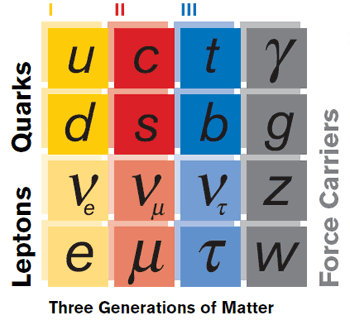
\includegraphics[width=360pt]{Figures/theory-standard-model-symmetry-mag.png}
    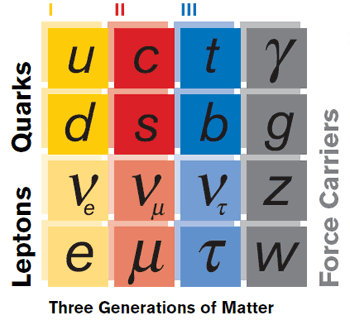
\includegraphics[width=240pt]{Figures/theory-standard-model-symmetry-mag.png}
  \end{center}
  \caption[\fixspacing Particles of the standard model]
	  {\fixspacing Known particles of the standard model, 
	    represented in three generations.
	  }
  \label{fig:StandardModel}
 \end{figure}


\begin{table}[htbp]
%  \centering
  \begin{center}
    \caption{\fixspacing Masses and charges of the Standard Model particles.}
    \label{TableSMParticles}
%    \begin{tabular}[]{ | l | c | c | }
    \begin{tabular}[]{ | c | c | c | c | c | c | }
      \hline
      Particle & Mass (GeV) & Charge (e) & Weak force & EM force & Strong force \\ \hline \hline
      \multicolumn{6}{|l|}{Quarks} \\ \hline 
      up, $u$ & $2.5 \times 10^{-3}$ & $+\frac{2}{3}$ & Yes & Yes & Yes \\ \hline
      down, $d$ & $5.0 \times 10^{-3}$ & $-\frac{1}{3}$ & Yes & Yes & Yes \\ \hline
      charm, $c$ & $0.10$ & $+\frac{2}{3}$ & Yes & Yes & Yes \\ \hline
      strange, $s$ & $1.29$ & $-\frac{1}{3}$ & Yes & Yes & Yes \\ \hline
      top, $t$ & $173$ & $+\frac{2}{3}$ & Yes & Yes & Yes \\ \hline
      bottom, $b$ & $4.2$ & $-\frac{1}{3}$ & Yes & Yes & Yes \\ \hline
      \multicolumn{6}{|l|}{Leptons} \\ \hline
      electron, $e$ & $0.511 \times 10^{-3}$ & $-1$ & Yes & Yes & No \\ \hline
      muon, $\mu$ & $106 \times 10^{-3}$ & $-1$ & Yes & Yes & No \\ \hline
      tau, $\tau$ & $1.78$ & $-1$ & Yes & Yes & No \\ \hline
      electron neutrino, $\nu_e$ & $< 2 \times 10^{-6}$ & $0$ & Yes & No & No \\ \hline
      muon neutrino, $\nu_{\mu}$ & $< 2 \times 10^{-6}$ & $0$ & Yes & No & No \\ \hline
      tau neutrino, $\nu_{\tau}$ & $< 2 \times 10^{-6}$ & $0$ & Yes & No & No \\ \hline
      \multicolumn{6}{|l|}{Bosons} \\ \hline
      photon, $\gamma$ & 0 & $0$ & No & No & No \\ \hline
      $W\pm$ & 80.4 & $\pm 1$ & No & Yes & No \\ \hline
      $Z$ & 91.2 & $0$ & No & No & No \\ \hline
      gluon, $g$ & 0 & $0$ & No & No & Yes \\ \hline
    \end{tabular}
  \end{center}
\end{table}


\subsection{Particles}
\label{theory:particles}
%\section{quarks}
There are six ``flavors'' of quarks, 
often represented by their first letters: 
up, down, charm, strange, top, and bottom.  
The first quark in each pair has charge $+\frac{2}{3}$, 
%(in terms of the electron charge), 
while the second has charge $-\frac{1}{3}$.  
These charges are given in terms of the electron charge; 
though the charges are fractional, 
the quarks are always arranged into composite 
particles that have integer multiples of the electron charge.  
These composite particles are known as ``hadrons'' 
and are divided into two categories: 
``mesons,'' made of a quark and an antiquark, 
and ``baryons,'' made of three quarks 
(or three antiquarks).  

%\section{leptons}
The leptons consist of the electron, muon, and tau ($\tau$), 
each with charge -1, 
and their corresponding neutrinos, 
the electron neutrino, muon neutrino, and $\tau$ neutrino, 
which are chargeless.  
Until recently it was believed that all the neutrinos are massless.  
However, recent experiments indicate 
that neutrinos do have a small mass 
\cite{neutrinoMixing}.  

%\section{bosons}
The bosons in the last column transmit the forces 
by which particles interact.  
%The massless photon ($\gamma$) and gluon ($g$) 
%transmit the electromagnetic and the strong forces, 
%respectively, 
The massless photon ($\gamma$) transmits the 
electromagnetic (EM) force; 
this particle is more familiar in its 
everyday context as the particle that makes up light.  
The gluon ($g$), also massless, transmits the strong force, 
which holds protons and neutrons together     %%%%%% STRENGTH OF FORCES, mass of propagator?? but not in all cases
(like glue, hence the name).  
The relatively heavy $Z$ and $W$ bosons 
transmit the weak force, 
which causes nuclear decay.  
Each force has an intrinsic strength, % characteristic
represented by its ``coupling constant.''  
The strong force's coupling constant ($\alpha_S$)
is larger than that 
of the electromagnetic force ($\alpha$); 
the weak force's ($G_F$) is weaker.  

%\section{antiparticles}
In general, each particle has an antiparticle partner, 
often denoted by a bar ($\bar{u}$), 
of the opposite charge and quantum numbers; % opposite quantum numbers in general, explain quantum numbers? because have to account for photon, gluon, Z, neutrinos
quantum numbers are used to describe the properties of the particles 
and corresponding interactions.  
For instance, all leptons have a non-zero ``lepton number;'' 
if the initial state of a set of particles 
has a total lepton number of 1, 
then any interaction between those particles will 
result in a final state with the same lepton number.  
Lepton number is always conserved in this way, 
as are charge and other quantum numbers.  
The antiparticle of the electron ($e^-$) 
has the opposite charge and lepton number 
and is called the positron ($e^+$).  
Neutrinos, being chargeless, 
have antineutrinos with opposite lepton number.  
Quarks and gluons have another quantum ``number'' known as color.   
The three colors are red, green, and blue, with the corresponding 
``anti-colors'' being anti-red, anti-green, and anti-blue.  
%This ``color'' does not refer to our everyday experience of red, green, and blue, 
%%but there is a certain analogy to light in the ``quantum color'' behavior.  
%but the name is not accidental -- there is an analogy to colored light.  
Color is unique in that all observed states of quarks and gluons 
are ``colorless.''
In two-quark states, a color and its anti-color ``combine'' to make a colorless state.  
Three-quark states are also colorless, but through a different combination: 
the three quarks are colored red, green, and blue 
(or the corresponding anticolors), which ``combine'' (like colored light) to form 
a state with no color
In practice, antiparticles are often called by their particle names; 
since it is known that a neutral Z must decay to one positive and one negative 
particle, no distinction is made between ``positron'' and ``electron'' -- 
both are called ``electrons.''  

%\section{higgs}  
Not shown in Figure~\ref{fig:StandardModel} is the Higgs boson, 
which is predicted by the Standard Model 
to give mass to the other particles.  
The Higgs has not yet been discovered; 
finding it (if it exists) is one of the 
goals of the LHC.  

%\section{gravity}
The Standard Model does not include the final 
fundamental force, gravity.  
Gravity is the weakest of the forces and does not 
measurably affect interactions between fundamental particles.  
The reason that it is the only one observable on a 
cosmological scale is because its ``charge,'' mass, 
is cumulative; there is no anti-mass to counter it 
the way a negatively-charge electron and a positively-charged 
proton combine to make an electrically neutral hydrogen atom.  
Gravity has been described on a macroscopic scale, but 
so far no theory has fully united gravity with the 
other fundamental forces.  
%There are many efforts currently ongoing to unite them, % REFERENCE?
%but none of these approaches have yet been proved.  
Such a ``theory of everything'' is 
%a dream of 
one of the goals that 
theoretical physics %.  
pursues.  





%\section{forces and groups?}
\subsection{Forces}
\label{theory:ForcesGroups}
%gauge groups, little intro to group theory

The forces in the Standard Model can be described 
by group mathematics.  
A ``group'' is a set of elements with specific properties.  
In particular, a transformation applied to an element in the group 
results in another element in the group.  
A ``Lie'' group is one in which any transformation % NEED THIS????
can be done in very small steps, 
each of which results in an element still in the group.  
The different fundamental forces are 
each described by such a Lie group.  
%which particles feel which forces?
%Each of the three forces in the Standard Model 
%is described by such a Lie group.  % group. 
%In each case, the ``dimension'' of the group 
%is the dimension of the matrices
Each group is represented by a set of square matrices 
of some dimension, given by the number in parentheses 
in the name of the group.  
The matrices used for these representations are 
all unitary (hence the common ``U'' designation).  
``Unitary'' means that the matrix's inverse 
is equal to its complex conjugate transpose.  
In other words, if you flip the matrix's elements 
about its diagonal and replace each imaginary unit $i$ 
with $-i$, then multiply it by the original matrix, 
the result is the identity matrix.   % EXPLAIN IDENTITY MATRIX??

\subsubsection{Electromagnetic Force}
%\subsubsection{EM: U(1)}
\label{theory:EM}
The electromagnetic force is described by the $U(1)$ group.  
Essentially, this describes rotation about an axis.  % talk about more than matrices?
The single parameter (an angle) requires only one matrix, 
corresponding to a single % force particle(s)
force carrier, the photon.  
The electromagnetic force causes interactions between 
photons and any particles that have electric charge.  
This includes quarks, leptons, and the charged weak bosons.  
%Because the photon is massless, the electromagnetic force % EXPLAIN MORE???
%can act over long distances, observable on the human scale.  

%\subsubsection{Weak: SU(2)}
\subsubsection{Weak Force}
\label{theory:weak}
The weak force is represented by the $SU(2)$ group.  
The ``S'' addition in the name stands for ``special'' 
and means that each matrix's trace 
(the sum of elements along the matrix's diagonal) is zero.  
$SU(2)$ represents rotations in three dimensions 
using three matrices, 
and therefore has three parameters corresponding 
to the single angle of $U(1)$.  
These give rise to the three carriers of the weak force, 
the two oppositely-charged W's and the Z.  %%% FIGURE OUT HOW TO DO W+- in latex? sort of like writing it out longhand, but should show at least W+ and W- notation 
%All three carriers have significant mass, which means 
%the distance over which they have an effect is very small.  
The weak force acts on any particles that have the ``weak 
version'' of electrical charge, %known as %``hypercharge.''  
%``weak isospin.''
namely all fermions.  
%All fermions interact via the weak force; 
In particular, the weak force is the only way 
neutrinos interact.  
%However, interactions with W's only happen in ways  % TALK ABOUT CONSERVATION OF CHARGE IN GENERAL
%that conserve charge.  
%Hypercharge is a combination of electric charge 
%and weak isospin.  

%\subsubsection{QCD: SU(3)}
\subsubsection{Strong Force}
\label{theory:strong}
Finally, the strong force is represented by $SU(3)$, 
which does not have an easy analogy to rotations 
like the previous two groups.  
It uses eight matrices, which correspond to the 
eight different gluon states that mediate the force.  
% talk about dim-3 = 3 colors?
The three dimensions of the group relate to the 
three ``color charges,'' red, green, and blue.  
Strong force interactions happen between all particles 
that carry this color charge, 
namely quarks, but also gluons themselves.  
% talk about color confinement and asymptotic freedom?  YES, but how to explain in terms of mass???
This so-called self-interaction on the part of the gluons 
causes the strong force to increase with distance.  
At short distances, the quarks making up another particle 
essentially act free; 
only when they get further apart do they feel the force 
keeping them in their bound state.  
This situation is related to the fact that quarks are 
never observed alone, only within these bound states.  
An interaction that is energetic enough to cause 
quarks to separate is also energetic enough to 
create more quarks with which the original quarks 
form new bound states.  
%When a quark gains a significant energy 
%(through an interaction with another particle), 

%This is known as color confinement
%The implication is that in spite of the fact that 
%gluons are massless, 
%the strong force is not observable over large distances.  

\subsection{Parton Distribution Functions}
\label{theory:pdf}

Since quarks do not exist in an isolated state 
outside hadrons, 
any interaction between them must also take 
into account the structure of thosee hadrons, 
in this case protons.  
The quark structure of protons is given 
by a set of functions called 
``parton distribution functions'' or PDFs, 
$f_i(x)$. 
%\[
%f_i(x)
%\]
These functions represent the probability 
of finding a given quark flavor $i$ inside 
the proton with a given momentum.  
The quark's momentum itself is not used; 
rather, the fraction of the proton's 
momentum that the quark carries, or $x$. 
Since no quark can have momentum greater 
than that of the proton itself, 
the value of $x$ ranges from 0 to 1.  
%Furthermore, % do PDFs only refer to quarks??? do they necessarily integrate to 1??
A proton is said to consist of two up quarks 
and a down quark; 
however, these represent the ``valence'' quarks only.  
A ``sea'' of quarks is also present, 
formed from gluons and each existing only 
momentarily, 
illustrated in Figure~\ref{fig:ProtonQuarkModel}.  
Therefore the PDFs represent all quark 
flavors, not just $u$ and $d$.  

%QUARK MODEL PICTURE

 \begin{figure}[htb]
  \begin{center}
%    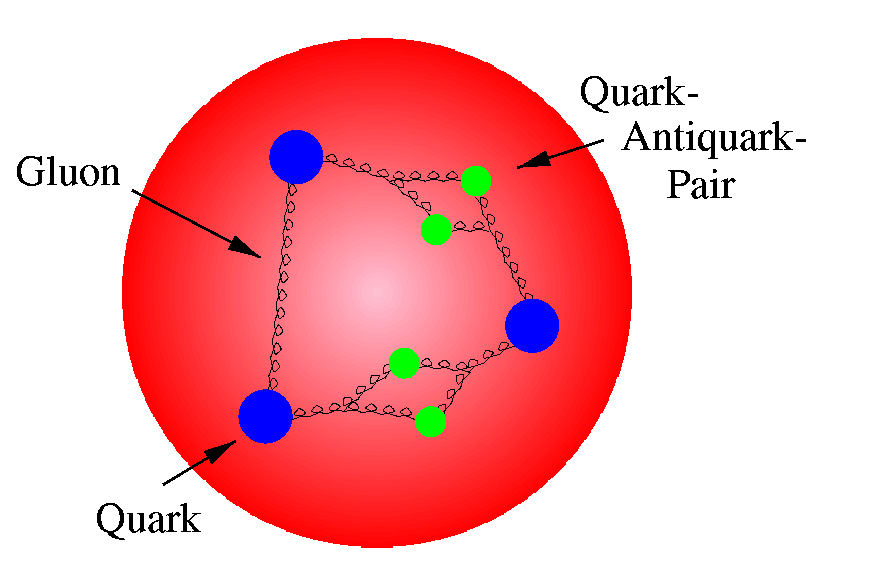
\includegraphics[width=360pt]{Figures/theory-quark-proton-naif-desy.png}
    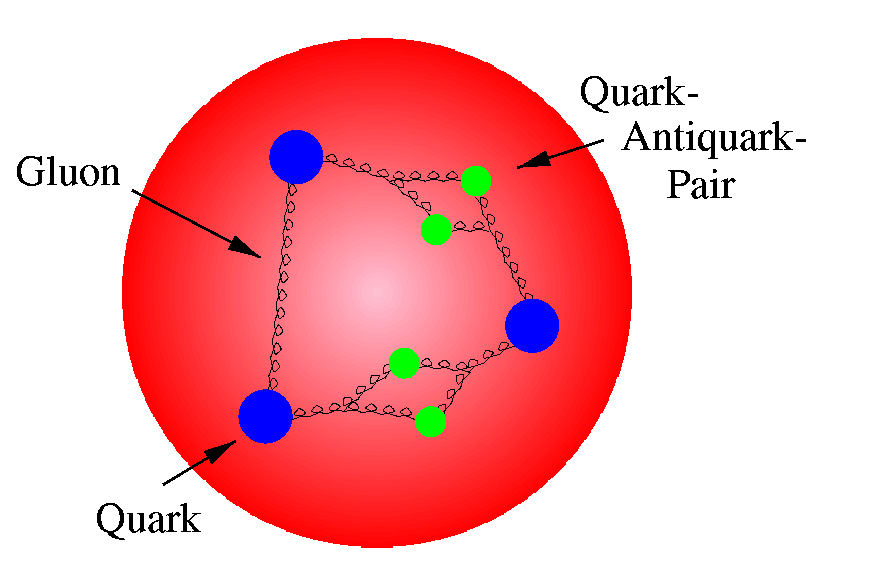
\includegraphics[width=240pt]{Figures/theory-quark-proton-naif-desy.png}
  \end{center}
  \caption[\fixspacing Quark model of proton]
	  {\fixspacing Quark model of the proton, 
	    showing the three valence quarks 
	    and the quark-antiquark pairs 
	    that make up the quark sea. 
	  }
  \label{fig:ProtonQuarkModel}
 \end{figure}



PDFs cannot be calculated from first 
principles and must be measured by fits 
to experimental data.  
There are several independent sets of PDFs 
in distribution.  
The simulated signal sample used in this analysis 
were generated with the CT10 PDF set \cite{CT10}, 
while the theoretical cross section calculation 
used the MSTW set \cite{MSTW}.  
The background samples used a slightly older 
version of CT10 called CTEQ6L1 \cite{CTEQ6L1}. 
The currently-distributed PDF sets 
account for data from all major past experiments.  
However, there is still some uncertainty, 
%in the PDFs, 
and precision measurements of Z production 
at the LHC can %help %contribute to better PDF sets.  
improve the community's knowledge of PDFs.  



%% \section{Electroweak Physics}
%% \label{theory:EWK}

%\section{ewk: SU(2)xU(1)}
\subsection{Electroweak Physics}
\label{theory:EWK}
The forces here have been given in terms 
of mathematical groups.  
However, the individual groups by themselves 
do not necessarily represent the reality of particles.  
It is known experimentally that the bosons carrying 
the weak force have mass.  
%The $SU(2)$ formulation of the weak force
In order for the theory to correctly predict the 
fact those particles should be massive, 
the electromagnetic and weak interactions had to be combined 
into a single framework, 
%Steven Weinberg and Abdus Salam 
%The electromagnetic and weak forces were combined into one framework, 
$SU(2) \times U(1)$, using a specific method.  
The integrated $SU(2) \times U(1)$ group 
allows for the collective four force-carrying bosons 
(photon, positively- and negatively-charged W's, and Z) 
to be described as compositions of the same underlying states.  
The elecroweak interaction has its own set of quantum 
numbers: ``weak isospin,'' and ``hypercharge,'' 
which combines weak isospin with electric charge.  
$T_3$ is the third component of the isospin 
and relates how to the fermions are arranged 
within the standard model generations 
(refer to Figure~\ref{fig:StandardModel}).  
Each generation consists of two pairs, 
one pair of quarks and one pair of leptons.  
The placement of each particle within its pair 
reflects how it interacts with the weak force.  
%This quantity is the ``weak version'' of electric charge, 
%known as ``hypercharge.''  
For the top particle in each pair, the hypercharge 
is $+\frac{1}{2}$; 
for the bottom particle, it is $-\frac{1}{2}$.  
(Note: this only applies to particles whose spin 
is ``left-handed,'' 
or oriented to spin left with respect to its direction of motion.  
Particles with ``right-handed'' spin have zero weak isospin; 
right-handed neutrinos do not interact in the Standard Model.  
This is equivalent with the assertion that neutrinos 
must be moving at the speed of light and therefore 
do not have mass. 
If neutrinos had mass, 
they would be moving slower than the speed of light 
and there could be a reference frame -- 
where the observer moves faster than the neutrino -- 
in which the neutrino would actually be left-handed.  
Because recent observations have indicated neutrinos % REFERENCE
do in fact have mass, 
this aspect of the Standard Model is inaccurate.)  

\subsubsection{Spontaneous Symmetry Breaking}
\label{theory:SpontSymmBreak}
The fact that the three weak bosons are massive, though, 
comes from applying ``spontaneous symmetry breaking.''  
This method uses the fact that the groups mentioned 
above have underlying symmetries: 
that is, they contain parameters that do not affect the 
physical description in any way.  
They are symmetric with respect to variations in these parameters.  
However, the values of these parameters can be chosen 
in a strategic way and the result manipulated % TALK ABOUT FIELD THEORY AT ALL?? this is all lagrangians and mass terms
to give masses to the weak bosons.  
(A consequence of this ``strategic choice'' is the appearance 
of another massive particle in the theory: 
the Higgs boson.  
The Higgs boson is therefore predicted by the theoretical 
mechanism used to account for massive weak bosons.  
Time -- and collision data -- will tell if the theory 
in this form is correct.)  


\section{Z Production}
\label{theory:Zprod}

Theoretical treatment of Z production 
requires a wide variety of tools.  
The following sections attempt to introduce 
and explain those concepts, 
arriving at a discussion of the 
cross section calculation.  

\subsection{Relativistic Kinematics}
\label{theory:RelKin}
A particle's coordinates can be described in terms of 
four quantities: its three spatial coordinates 
and its point in time.  This is conventionally 
represented as 
\[
x^{\mu} = (t, x, y, z)
\]
(where we are treating the speed of light to be 
equal to 1).  
A particle (or everyday object) can appear to 
have different properties of motion 
depending on the reference 
frame from which it is viewed.  
If you are sitting on an airplace at cruising altitude, 
the plane is not moving with respect to your body.  
However, if you are on the ground, the plane is 
moving very fast. % -- 
%it has a different kinetic energy in that frame.  
The physics of the situation cannot depend on 
the reference frame of the observer, 
even at the relativistic speeds of interacting particles.  
%Moving at relativistic speeds, 
%or being viewed from a relativistic reference frame, 
%can change the relation between these 
%four quantities at any point.  
There is, however, a certain combination 
of those time and position coordinates that is 
%However, a certain combination is 
invariant -- that is, it remains the same no 
matter the speed or reference frame.  
This invariant can be constructed as 
\[
t^2 - x^2 - y^2 - z^2 = x^{\mu} x_{\mu}
\]

In the same way, a particle's motion can be described 
in terms of its energy and the three components of 
its momentum, called ``four-momentum:''
\[
p^{\mu} = (E, p_x, p_y, p_z)
\]
The invariant combination is called ``invariant mass'' 
and is equal to the particle's rest mass.  
%
%% %PUT INV MASS UP HERE
%% %\section{inv mass}
%% %The definition of a 
%% A particle system's ``invariant mass'' is 
%% a combination of its energies and momenta that 
%% remain unchanged regardless of reference frame.  
%
%% The invariant mass is such a quantity that 
%% remains the same.  
In addition, since the energy and momentum 
of a system are conserved, 
the invariant mass is also conserved 
throughout the entire interaction, 
in particular the decay.  
The general definition is given by 
\[
p^{\mu}p_{\mu} = M_{inv}^2 = \left( \sum E \right)^2 - \left\| \sum \mathbf{p} \right\|^2
\]
or
\[
M_{inv} = \sqrt{ \left( \sum E \right)^2 - \left\| \sum \mathbf{p} \right\|^2 }
\]
For a single particle, the expression simplifies 
to the particle's mass.  
This analysis makes use of the fact that the 
invariant mass of the decay particles 
(the two electrons) 
is the same as the (invariant) mass of the 
particle which decayed, the Z.  
The above formula, simplified to two particles, 
\[
M_{inv} = \sqrt{ \left(E_1 + E_2\right)^2 - \left\|\mathbf{p}_1 + \mathbf{p}_2\right\|^2 }
\]
reconstructs the mass of the Z boson 
based on the energies and momenta 
of the decay products.  
%The Z's $M_{inv}^2$ is also the energy 
%of the interaction, $\hat{s}$ 
%(see Section~FIXME).  

%\section{kinematics like s}
It is also useful to define variables 
characterizing the collision itself.  
The quantity $s$ is the square of the center-of-momentum 
energy of the colliding proton system.  
(Therefore $\sqrt{s}$ is the center-of-momentum 
energy itself.)  
It is obtained by adding together the four-momenta 
of the colliding protons, designated $1$ and $2$: %.  
\[
s = (p_1 + p_2)^2
\]
However, since only a single quark participates 
in the interaction, not the full proton, 
the energy of the interaction must be reduced.  
Since $x$ the fraction of the proton's momentum that is carried 
by the quark (see Section~\ref{theory:pdf}), %is defined $x$, so that 
the 
quark's momentum is then $xp$.  
We can then define a center-of-momentum energy, 
$\hat{s}$ (or $Q^2$), 
for the quark-quark system, 
the interacting part of the proton system: 
\[
\hat{s} = (x_1 p_1 + x_2 p_2)^2 = Q^2
\]
($\hat{s}$ and $Q^2$ will be used interchangeably.)  
This can be approximated in terms of the original 
(proton) $s$ as 
\[
\hat{s} \simeq x_1 x_2 s
\]
In a center-of-momentum frame, $\hat{s}$ is equal 
to the invariant mass of the quark pair, 
and therefore, the mass of the Z that is produced.  



\subsection{Feynman Diagrams}
\label{theory:feynman}
% MOVE THIS SECTION????

%Transformations within these groups can be represented as matrices.  % IS THIS ACTUALLY THE SAME AS THE GROUP MATRICES??
The concept of matrices that 
transform a particle's state 
was introduced in Section~\ref{theory:ForcesGroups}. 
Matrices are often used to represent transitions 
from one quantum mechanical state to another.  
This can be broadened to the full interaction.  
Such a matrix acts on the set of initial states 
and result in the set of final states.  
Each element in the matrix, mapping an initial state 
to a final state, 
gives the amplitude with which the % ONLY IN SCATTERING???  make sure this is right context 
transformation happens.  
Essentially, squaring the matrix element gives the 
relative probability of that particular transformation.  

This is used in particle physics as such: 
a transformation from an initial state, 
in our case two quarks from colliding protons, 
to a final state, 
an electron and a positron, 
is represented by a Feynman diagram, 
shown in Figure~\ref{fig:ZeeFeynmanDiagram}.  
The interaction can be thought to progress to the right.  
Each straight line represents a fermion, 
either the quark or the electron.  
The wavy line represents a boson, the Z.  
(Gluons are represented by curly lines.)  
The intersections between particle lines, or vertices, 
show interactions between the given particles.  
%The type of interaction can be determined by the particles   % NEED THIS?  
%taking part: 
%an interaction between a Z and a quark or lepton 
%indicates the weak force is involved.  
The matrix element corresponding to this transformation 
can be written down 
by attributing factors to the various elements 
of the Feynman diagram: 
the particle lines and the vertices.  
In this way, the diagrams are not just useful 
conceptual pictures 
but also powerful calculational tools.  
%somewhere get into spinors...

%put equation for differential cross section element 
%in terms of amplitude/matrix element 

\begin{figure}[htb]
\begin{center}
  \begin{tikzpicture}[
      thick,
      % Set the overall layout of the tree
%      level/.style={level distance=1.4cm, line width=0.8mm},
      level/.style={level distance=1.4cm, line width=0.5mm},
      level 2/.style={sibling distance=1.4cm},
      level 3/.style={sibling distance=1.4cm}
    ]
    \coordinate
%    child[grow=south east]{
%      child[grow=north east]{
%        edge from parent [gluon]
%        node[right]{$g$}
%      }
    child[grow=south east]{
      edge from parent [electron]
      child[grow=south west] {
        edge from parent [electron]
%        node[above] {$\bar{q}$} % ADDED
        node[below] {$\bar{q}$} % ADDED
%          child[grow=south west]{
%            edge from parent [electron]
%            node[above] {$\bar{q}$}
%          }
%          child[grow=south east]{
%            edge from parent [gluon]
%            node[right] {$g$}
%          }
      }
      child[grow=east, level distance=2.4cm] {
        child[grow=south east]{ % added the [], did nothing, don't know how to make angle of line the same as LHS
          edge from parent [electron]
          node[below] {$e^{-}$}
        }
        child[grow=north east]{ % added the [], did nothing, don't know how to make angle of line the same as LHS
          edge from parent [electron]
          node[above] {$e^{+}$}
        }
        edge from parent [boson]
%        edge from parent [zboson]
%        node[below] {$Z/\gamma*$}
        node[below] {$Z$}
      }
%    }
      edge from parent [electron] node [above=3pt] {$q$}
    };
  \end{tikzpicture}
\end{center}
%  \caption[Feynman diagram of \qqZgee]
  \caption[\fixspacing Feynman diagram of \qqZee]
%	  {Feynman diagram of \qqZgee.  
	  {\fixspacing Feynman diagram of \qqZee.  
	    }
  \label{fig:ZeeFeynmanDiagram}
\end{figure}

\subsection{Interference from $q \bar{q} \rightarrow \gamma* \rightarrow e^+ e^-$}
\label{theory:DY}
In this case, another diagram contributes 
to the process being studied: 
a photon replaces the Z boson 
as the link between the quarks and the electrons.  
This is known as the Drell-Yan process.
Both cases are illustrated in 
Figure~\ref{fig:ZeeFeynmanDiagramZ}. 
Because these diagrams have the exact same 
initial and final states, 
they ``interfere'' with each other.  
Experimentally, it is impossible to tell which one happened; 
both must be included in the calculations.  % is this exactly why???

%BOTH DIAGRAMS SIDE-BY-SIDE
% DOUBLE PICTURE!
\begin{figure}[htb]
\begin{center}
  \subfloat[]{
    \begin{tikzpicture}[
	thick,
	% Set the overall layout of the tree
	%      level/.style={level distance=1.4cm, line width=0.8mm},
	level/.style={level distance=1.4cm, line width=0.5mm},
	level 2/.style={sibling distance=1.4cm},
	level 3/.style={sibling distance=1.4cm}
      ]
      \coordinate
      %    child[grow=south east]{
      %      child[grow=north east]{
      %        edge from parent [gluon]
      %        node[right]{$g$}
      %      }
      child[grow=south east]{
	edge from parent [electron]
	child[grow=south west] {
          edge from parent [electron]
	  %        node[above] {$\bar{q}$} % ADDED
          node[below] {$\bar{q}$} % ADDED
	  %          child[grow=south west]{
	  %            edge from parent [electron]
	  %            node[above] {$\bar{q}$}
	  %          }
	  %          child[grow=south east]{
	  %            edge from parent [gluon]
	  %            node[right] {$g$}
	  %          }
	}
	child[grow=east, level distance=2.4cm] {
          child[grow=south east]{ 
            edge from parent [electron]
            node[below] {$e^{-}$}
          }
          child[grow=north east]{ 
            edge from parent [electron]
            node[above] {$e^{+}$}
          }
	  edge from parent [boson]
          %edge from parent [zboson]
	  %        node[below] {$Z/\gamma*$}
          node[below] {$Z$}
	}
	%    }
	edge from parent [electron] node [above=3pt] {$q$}
      };
    \end{tikzpicture}
  \label{fig:ZeeFeynmanDiagramZ}
  }
  \subfloat[]{
    \begin{tikzpicture}[
	thick,
	% Set the overall layout of the tree
	%      level/.style={level distance=1.4cm, line width=0.8mm},
	level/.style={level distance=1.4cm, line width=0.5mm},
	level 2/.style={sibling distance=1.4cm},
	level 3/.style={sibling distance=1.4cm}
      ]
      \coordinate
      %    child[grow=south east]{
      %      child[grow=north east]{
      %        edge from parent [gluon]
      %        node[right]{$g$}
      %      }
      child[grow=south east]{
	edge from parent [electron]
	child[grow=south west] {
          edge from parent [electron]
          node[below] {$\bar{q}$} % ADDED
	  %          child[grow=south west]{
	  %            edge from parent [electron]
	  %            node[above] {$\bar{q}$}
	  %          }
	  %          child[grow=south east]{
	  %            edge from parent [gluon]
	  %            node[right] {$g$}
	  %          }
	}
	child[grow=east, level distance=2.4cm] {
          child[grow=south east]{ 
            edge from parent [electron]
            node[below] {$e^{-}$}
          }
          child[grow=north east]{ 
            edge from parent [electron]
            node[above] {$e^{+}$}
          }
	  edge from parent [boson]
	  node[below] {$\gamma*$}
	}
	%    }
	edge from parent [electron] node [above=3pt] {$q$}
      };
    \end{tikzpicture}
    \label{fig:ZeeFeynmanDiagramGamma}
  }
\end{center}
  \caption{\fixspacing Feynman diagrams for \qqZgee: 
    the $Z$ and $\gamma$ production interfere.}
  \label{fig:ZeeFeynmanDiagramCompare}
\end{figure}


It is necessary to note that the photon that takes 
part in this interaction is a ``virtual'' photon -- 
%it cannot be observed by itself.  
it cannot be directly observed.  
The reason for this is that there is always a 
center-of-momentum reference 
frame for the two particles colliding to form the photon.  
In other words, there is always some way that you, 
the observer, can be moving, 
such that it looks like the two particles 
have the same speed but opposite directions.  
In this reference frame, the photon would be formed at rest, 
which violates the principle that the speed of light 
is the same in all reference frames -- 
the speed of light can never be zero.  
Equivalently, such a photon would have mass, 
while real photons are massless.  
The mass of this virtual photon is indeed the same 
as the invariant mass of the system.  
%Such virtual particles can exist due to inherent   %% is that actually why these photons in particular can be virtual?  
%fluctuations in energy, by the uncertainty 
%principle of quantum mechanics.  
Such virtual particles are allowed to exist 
by the uncertainty principle of quantum mechanics, 
which governs the ``borrowing'' of energy from the vacuum.  
The smaller the time scale over which the energy 
fluctuation happens, 
the larger the energy fluctuation allowed.  

\subsection{Mass Distribution}
\label{theory:mass}
Having a specific mass defines a thin 
surface or ``shell'' in kinematic phase space; 
only certain combinations of energy and momentum 
are allowed, 
because of the relations between mass, energy, and momentum.  
Particles that are virtual, 
i.e. have a mass much different than their 
defined ``real'' mass, 
are called ``off-shell'' -- 
they are ``off the mass shell.''  

%\section{Z can be offshell like photon, that's why it's a distribution with a peak with a width}
The Z boson, while it has a defined mass, 
%DECAY WIDTH ETC ETC ETC 
can be ``off-shell'' in the same way as the photon.  
That is, in general the 
%reconstructed 
mass 
does not take on a single precise value; 
instead, over many events it manifests as a distribution 
peaked around the ``real'' value.  
This is typical of particles that are measured only 
by their decays, called ``resonances;'' 
these particles tend to be at least slightly virtual 
%because they are not being observed directly.  
because of their short lifetimes.  
%in fact, 
%\section{decay lifetime partial width}
In addition, the width of the peak is inversely proportional to the 
lifetime of the particle.  
The wider the peak, the more final states the particle can decay into, 
and the more likely it is to decay.  
The contribution of each final state is called the 
``partial width;'' 
this quantity plays a role in calculating 
how often a given resonance is produced.  




\subsection{Higher-Order Diagrams}
\label{theory:HigherOrderDiagrams}
%put all qcd stuff in here?  don't need all the detail of zeus stuff

%NOT JUST QCD!  vertices in QED, too!  

In real life a given interaction is 
never represented by just a finite set of diagrams.  
For each simple diagram, 
such as Figure~\ref{fig:ZeeFeynmanDiagram}, 
there is an infinite number of 
more-complicated diagrams that 
represent the same initial and final states.  
A few examples are illustrated in 
Figure~\ref{fig:ZeeFeynmanDiagramHighOrder}.  

%FIGURE WITH MORE FEYNMAN DIAGRAMS
% DOUBLE PICTURE!
\begin{figure}[htb]
\begin{center}
%%   \subfloat[]{
%%     \begin{tikzpicture}[
%% 	thick,
%% 	% Set the overall layout of the tree
%% 	%      level/.style={level distance=1.4cm, line width=0.8mm},
%% 	level/.style={level distance=1.4cm, line width=0.5mm},
%% 	level 2/.style={sibling distance=1.4cm},
%% 	level 3/.style={sibling distance=1.4cm}
%%       ]
%%       \coordinate
%%       %    child[grow=south east]{
%%       %      child[grow=north east]{
%%       %        edge from parent [gluon]
%%       %        node[right]{$g$}
%%       %      }
%%       child[grow=south east]{
%% 	edge from parent [electron]
%% 	child[grow=south west] {
%%           edge from parent [electron]
%% 	  %        node[above] {$\bar{q}$} % ADDED
%%           node[below] {$\bar{q}$} % ADDED
%% 	  %          child[grow=south west]{
%% 	  %            edge from parent [electron]
%% 	  %            node[above] {$\bar{q}$}
%% 	  %          }
%% 	  %          child[grow=south east]{
%% 	  %            edge from parent [gluon]
%% 	  %            node[right] {$g$}
%% 	  %          }
%% 	}
%% 	child[grow=east, level distance=2.4cm] {
%%           child[grow=south east]{ 
%%             edge from parent [electron]
%%             node[below] {$e^{-}$}
%%           }
%%           child[grow=north east]{ 
%%             edge from parent [electron]
%%             node[above] {$e^{+}$}
%%           }
%% 	  edge from parent [boson]
%%           %edge from parent [zboson]
%% 	  %        node[below] {$Z/\gamma*$}
%%           node[below] {$Z$}
%% 	}
%% 	%    }
%% 	edge from parent [electron] node [above=3pt] {$q$}
%%       };
%%     \end{tikzpicture}
%% %  \label{fig:ZeeFeynmanDiagramZ}
%%   }
  \subfloat[]{
    \begin{tikzpicture}[
	thick,
	% Set the overall layout of the tree
	%      level/.style={level distance=1.4cm, line width=0.8mm},
%	level/.style={level distance=1.4cm, line width=0.5mm},
	level/.style={level distance=1.0cm, line width=0.5mm},
%	level 2/.style={sibling distance=1.4cm},
	level 2/.style={sibling distance=1.0cm},
%	level 3/.style={sibling distance=1.4cm}
	level 3/.style={sibling distance=1.0cm}
      ]
      \coordinate
      %    child[grow=south east]{
      %      child[grow=north east]{
      %        edge from parent [gluon]
      %        node[right]{$g$}
      %      }
      child[grow=south east, level distance=2.0cm]{
	edge from parent [electron]
	child[grow=south west, level distance=2.0cm] {
          edge from parent [electron]
          node[below] {$\bar{q}$} % ADDED
	  %          child[grow=south west]{
	  %            edge from parent [electron]
	  %            node[above] {$\bar{q}$}
	  %          }
	  %          child[grow=south east]{
	  %            edge from parent [gluon]
	  %            node[right] {$g$}
	  %          }
	}
	child[grow=east, level distance=2.4cm] {
          child[grow=south east]{ 
            child[grow=south east]{ 
              edge from parent [electron]
              node[below] {$e^{-}$}
	    }
          }
          child[grow=north east]{ 
            child[grow=south east]{ 
              edge from parent [boson]
              node[above] {$\gamma$}
	    }
            child[grow=north east]{ 
              edge from parent [electron]
              node[above] {$e^{+}$}
	    }
          }
	  edge from parent [boson]
	  node[below] {$Z$}
	}
	%    }
	edge from parent [electron] node [above=3pt] {$q$}
      };
    \end{tikzpicture}
%    \label{fig:ZeeFeynmanDiagramGamma}
  }
  \subfloat[]{
    \begin{tikzpicture}[
	thick,
	% Set the overall layout of the tree
	%      level/.style={level distance=1.4cm, line width=0.8mm},
%	level/.style={level distance=1.4cm, line width=0.5mm},
	level/.style={level distance=1.0cm, line width=0.5mm},
%	level 2/.style={sibling distance=1.4cm},
	level 2/.style={sibling distance=1.0cm},
%	level 3/.style={sibling distance=1.4cm}
	level 3/.style={sibling distance=1.0cm}
      ]
      \coordinate
      %    child[grow=south east]{
      %      child[grow=north east]{
      %        edge from parent [gluon]
      %        node[right]{$g$}
      %      }
      child[grow=south east, level distance=2.0cm]{
	edge from parent [electron]
	child[grow=south west, level distance=2.0cm] {
          edge from parent [electron]
          node[below] {$\bar{q}$} % ADDED
	  %          child[grow=south west]{
	  %            edge from parent [electron]
	  %            node[above] {$\bar{q}$}
	  %          }
	  %          child[grow=south east]{
	  %            edge from parent [gluon]
	  %            node[right] {$g$}
	  %          }
	}
	child[grow=east, level distance=2.4cm] {
          child[grow=south east]{ 
            child[grow=south east]{ 
              edge from parent [electron]
              node[below] {$e^{-}$}
	    }
          }
          child[grow=north east]{ 
            child[grow=south, level distance=1.4cm]{ 
              edge from parent [boson]
              node[right] {$\gamma$}
	    }
            child[grow=north east]{ 
              edge from parent [electron]
              node[above] {$e^{+}$}
	    }
          }
	  edge from parent [boson]
	  node[below] {$Z$}
	}
	%    }
	edge from parent [electron] node [above=3pt] {$q$}
      };
    \end{tikzpicture}
%    \label{fig:ZeeFeynmanDiagramGamma}
  }
  \subfloat[]{
    \begin{tikzpicture}[
        thick,
        % Set the overall layout of the tree
%        level/.style={level distance=1.4cm, line width=0.5mm},
        level/.style={level distance=1.0cm, line width=0.5mm},
%        level 2/.style={sibling distance=1.4cm},
        level 2/.style={sibling distance=1.0cm},
%        level 3/.style={sibling distance=1.4cm}
        level 3/.style={sibling distance=1.0cm}
      ]
      \coordinate
      child[grow=south east]{
        child[grow=north east]{
          edge from parent [gluon]
          node[right=3pt]{$g$}
        }
        child[grow=south east]{
          edge from parent [electron]
          child[grow=south west] {
            edge from parent [electron]
            child[grow=south west]{
              edge from parent [electron]
              node[above] {$\bar{q}$}
            }
            child[grow=south east]{
              edge from parent [gluon]
              node[right=6pt] {$g$}
            }
          }
          child[grow=east, level distance=2.4cm] {
            child[grow=south east]{
              child[grow=south east]{
		edge from parent [electron]
		node[below] {$e^{-}$}
	      }
            }
            child[grow=north east]{
              child[grow=north east]{
		edge from parent [electron]
		node[above] {$e^{+}$}
	      }
            }
            edge from parent [boson]
            node[below] {$Z$}
          }
        }
        edge from parent [electron] node [above=3pt] {$q$}
      };
    \end{tikzpicture}
  }
  
\end{center}
  \caption{Higher-order Feynman diagrams for the process \qqZee.}
  \label{fig:ZeeFeynmanDiagramHighOrder}
\end{figure}


Fortunately, the more complicated a diagram, 
the smaller its contribution.  
Each vertex in the diagram contributes 
one factor of the relevant coupling constant. 
Since the coupling constants are small, 
a two-vertex diagram contributes much more 
than a three-vertex diagram, 
which contributes more than a 
four-vertex diagram, etc.  
%The number of vertices in a diagram 
However, the corrections from the higher-vertex 
(or ``higher-order'') 
diagrams make noticeable contributions 
to the overall result, 
and therefore they should be taken into 
account as far as possible.  
Commonly a particle in the initial or final state 
will radiate a photon or a gluon, 
creating another vertex.  
These particles will also produce a signature 
in the detector 
(the gluon after branching to quarks, 
which then continue to form 
a ``jet'' of hadrons, 
called ``hadronization''). 
These radiative processes are called 
``initial-state radiation'' (ISR) and 
``final-state radiation'' (FSR).  
Calculating the contributions from 
successively higher-order diagrams 
can be difficult, %though, 
and many specialized programs exist.  
(See Chapter~\ref{sim}.)  
The simplest Feynman diagram is called 
``leading order'' (LO), 
and the successively higher levels are 
``next-to-leading order'' (NLO) and 
``next-to-next-to-leading order'' (NNLO).  
This analysis uses a theoretical 
cross section calculation that 
was done in NNLO, 
which gives a result accurate to 
around 1\%.  



%lagrangian etc? i.e. more specifics on ewk physics

%feynman diagrams, how they can actually be used -> 
%matrix elements -> cross section element.  

%where to put cross section formula stuff 
%-- make new section?
%(and which stuff to use?)

%order of diagram = number of vertices!  

%someplace need to go into 4-momenta...

%s, inv mass, pdfs attach to tree-level matrix element, 
%Z/gamma* interference

%s = Z mass -- well, dunno, also includes momentum

\subsection{\Zee Cross Section}
\label{theory:xsec}

%!!!! THIS IS ALL FOR PHOTONS DRELL YAN !!!!!
%is that okay?????????
%Z's have different feynman rule factors!!


%more specific derivation stuff?  
%I guess, if I'm starting from the 
%feynman diagram stuff

The concept of the cross section was introduced previously, 
in terms of how to calculate it from experimentally-measured 
quantities.  
%Knowing the underlying physics, though, 
%the cross section can be calculated 
In principle, though, the cross section 
can also be calculated from the underlying physics.  
%The cross section can be expressed as 
%\[
%Cross section = \frac{W_{fi} }{\mathrm{initial flux}}
%\times (\mathrm{number of final states})
%\]
%$W_{fi}$ is the rate of transition from the initial state 
%to a given final state, expressed per unit volume.  
%The greater the number of possible final states, 
%the more likely a transition is to occur.  
The cross section element for a transition 
between two states can be expressed as 
% the VERY beginning of the cross section formula
% where |M|2 is ``probability'', F is flux = particles per area per time, 
% and dQ is dLIPS
\[
d \sigma = \frac{ \left| \mathcal{M} \right| ^2 }{F} d Q
\]
In this formula, $\mathcal{M}$ is the amplitude 
(or matrix element) governing the probability of 
transitioning from the initial state to the final state, 
$F$ is the particle flux, and $d Q$ is the 
phase space element.  
An initial state within the phase space element $d Q$ will 
contribute the element $d \sigma$ to the overall 
interaction cross section.  
Therefore, to get the full cross section, one must integrate 
over the full phase space.  
%Doing this in the center-of-momentum frame results 
%in the formula for the differential cross section 
For an interaction with two initial particles and 
two final particles 
(a $2 \rightarrow 2$ interaction), 
this can be integrated partially to 
% (in CM) the full differential cross section is 
% for any given feynman diagram
\[
\frac{d \sigma}{d \Omega} \bigg| _{CM} 
= \frac{1}{64 \pi^2 s} \frac{p_f}{p_i} \left| \mathcal{M} \right| ^2
\]
where $p_i$ and $p_f$ are the momenta of the initial and final particles 
(in the center-of-momentum frame with two particles, 
the initial and final momenta each have the same magnitude).  
Here $d \Omega$ is the solid angle element; 
the formula cannot be further integrated without knowing the 
(angular-dependent) form of $ \left| \mathcal{M} \right| ^2 $.  
% where d\Omega is solid angle element
% pf and pi are the initial and final momenta of each element,
% since in CM pi1 = pi2, pf1 = pf2
% differential is eventually integrated

%% % now for curly M squared
%% % Feynman diagram sez 
%% \[
%% \mathcal{M} = -
%% \]

%curly M can be written down from Feynman rules, 
%according to tensor structure

For any given Feynman diagram, 
such as Figure~\ref{fig:ZeeFeynmanDiagram}, 
a set of rules makes it possible to write 
down the elements of the interaction amplitude, 
$\left| \mathcal{M} \right| ^2$.  
%Due to the nature of electroweak interactions 
Electromagnetic interactions are fairly 
simple in structure and can be written down 
(and then calculated out) relatively easily.  
Electroweak interactions are somewhat 
more complicated.  
The full differential cross section for the interaction 
%the giant thing from the PDG RPP CH 40:
%while the giant thing is given by 
%(full differential cross section for 
%$ f_i \bar{f_j} \rightarrow (W,Z) \rightarrow f_{i'} \bar{f_{j'}} $
$ q_A \bar{q_B} \rightarrow Z \rightarrow e_{C} \bar{e_{D}} $
(where $q_A$ and $\bar{q_B}$ are the initial quarks 
and $e_{C}$ and $\bar{e_{D}}$ are the final electrons) is given by 
\cite{PdgRpp}
%\[
%\frac{d \sigma}{d \Omega} = \frac{N_c^f}{N_c^i} 
%\times \frac{1}{256 \pi s} 
%\times \frac{s^2}{(s - m_Z^2)^2 + s \Gamma^2}
%\times \left[(L^2 + R^2) (L'^2 + R'^2) (1 + \cos^2 \theta)
%+ (L^2 - R^2) (L'^2 - R'^2) 2 \cos \theta \right]
%\]
%Initial particles are quarks: 
%\[
%N_c^i = 3
%\]
%Final particles are leptons: 
%\[
%N_c^f = 1
%\]
%\[
\begin{align*}
%\frac{d \sigma}{d \Omega} (\qqZee) = \frac{1}{3} 
\frac{d \sigma}{d \Omega} 
( q \bar{q} \rightarrow Z \rightarrow e^+ e^- ) 
= &\frac{1}{3} 
\times \frac{1}{256 \pi s} 
\times \frac{s^2}{(s - m_Z^2)^2 + s \Gamma^2} \\
&\times \left[(L^2 + R^2) (L'^2 + R'^2) (1 + \cos^2 \theta)
+ (L^2 - R^2) (L'^2 - R'^2) 2 \cos \theta \right]
%\]
\end{align*}
$\Gamma$ is the \Zee decay's 
partial width (see Section~\ref{theory:mass}) 
given by %\cite{PdgRpp}
%% \[
%% \Gamma(Z \rightarrow f \bar{f} )
%% = N_c \frac{ \sqrt{2} G_F m_Z^3 }{6 \pi}
%% \times \left[(T_3 - Q_f \sin^2 \theta_W )^2 
%% + (Q_f \sin \theta_W )^2 \right]
%% \]
\[
\Gamma (Z \rightarrow e \bar{e} )
= \frac{ \sqrt{2} G_F m_Z^3 }{6 \pi}
\times \left[(T_3 - Q_f \sin^2 \theta_W )^2 
+ (Q_f \sin \theta_W )^2 \right]
\]
The $L$ and $R$ in the cross section equation 
refer to factors from %relating to the 
left-handed and right-handed initial quarks, respectively 
(likewise $L'$ and $R'$ refer to the final electrons).  
These factors are 
%For Z, couplings are 
\[
L = \sqrt{ \frac{8 G_F m_Z^2}{\sqrt{2} } }(T_3 - \sin^2 \theta_W Q)
%L = g (T_3 - \sin^2 \theta_W Q)
\]
\[
R = - \sqrt{ \frac{8 G_F m_Z^2}{\sqrt{2} } } \sin^2 \theta_W Q
%R = - g \sin^2 \theta_W Q
\]
%``$T_3$ is weak isospin of initial left-handed fermion and 
%Q is initial fermion's electric charge. [FRACTIONAL] 
%The expressions for L' and R' are analogous.  
%The color factors $ N_c^{i,f} $ are 3 for initial or final quarks 
%and 1 for initial or final leptons.''  
$T_3$ is the weak isospin of the left-handed particle 
(the right-handed particle has isospin 0, 
hence $T_3$ does not show up in $R$). 
$Q$ is the particle's electric charge.  
%BUT, initial particles are all flavors of quarks, 
%so can't just plug in flavor-dependent quantities 
%like $T_3$ and $Q$.  
%MUST SUM OVER FLAVORS.  oh boy!
The $T_3$ and $Q$ values for the relevant particles are 
given in Table~\ref{TableWeakNumbers}.  

%TABLE
\begin{table}[htbp]
%  \centering
  \begin{center}
    \caption{Charge and third component of weak isospin for 
      left-handed Standard Model fermions.}
    \label{TableWeakNumbers}
%    \begin{tabular}[]{ | l | c | c | }
    \begin{tabular}[]{ | l | c | c | }
      \hline
      Particle & $Q$ (e) & $T_3$  \\ \hline \hline
      $u,c,t$ & $+\frac{2}{3}$ & $+\frac{1}{2}$ \\ \hline
      $d,s,b$ & $-\frac{1}{3}$ & $-\frac{1}{2}$ \\ \hline
      $e,\mu,\tau$ & $-1$ & $+\frac{1}{2}$ \\ \hline
      $\nu_e, \nu_{\mu}, \nu_{\tau}$ & $0$ & $-\frac{1}{2}$ \\ \hline
    \end{tabular}
  \end{center}
\end{table}




Since the final-state particles are already known to be electrons, 
their values can be plugged into the equation.  
However, the flavor of the initial quarks is not known.  
Therefore, all the possible initial quark states must 
be taken into account, by adding up the contribution from each one.  

%H+M have SUCH a nice little summary in the inside back cover.  

%can put in terms of little g:
%\[
%g = \sqrt{ \frac{8 G_F m_Z^2}{\sqrt{2}} }
%\]


%% % WHICH simplifies to give us AVGD OVER SPINS or whatever
%% \[
%% \bar{ \left| \mathcal{M} \right| ^2 } 
%% = 2 e^4 \left[ \frac{1}{2} \left( 1 + \cos^2 \theta \right) \right]
%% \]

%% % THEN
%% \[
%% \frac{d \sigma}{d \Omega} \big| _{CM}
%% %= \frac{\alpha^2}{4s} \left( 1 + \cos^2 \theta \right) 
%% = \frac{\alpha^2}{4 Q^2} \left( 1 + \cos^2 \theta \right) 
%% \]


% quark-level subprocess is 3 e_q^2 times that for muons
% DON'T NEED TO SHOW THIS, backwards anyhow
%\[
%\sigma(e^- e^+ \rightarrow q \bar{q} ) 
%= 3 e_q^2 \sigma(e^- e^+ \rightarrow \mu^- \mu^+ )
%\]

%% % WHERE
%% %\[
%% %\sigma(e^- e^+ \rightarrow \mu^- \mu^+ ) 
%% %= \frac{4 \pi \alpha^2}{3 s}
%% %\]
%% % don't need to show that one either, 
%% %just result: 
%% \[
%% \sigma ( q \bar{q} \rightarrow e^- e^+ )
%% %= 3 e_q^2 \frac{4 \pi \alpha^2}{3 s}
%% = 3 e_q^2 \frac{4 \pi \alpha^2}{3 Q^2}
%% \]
%% % D'OH, look at next line!

%% % cross section of quark-level subprocess
%% \[
%% \hat{\sigma} (q \bar{q} \rightarrow l^- l^+) 
%% = \frac{4 \pi \alpha^2}{3 Q^2} e_q^2
%% \]

% but need to account for the proton and pdfs

The cross section for the photon process 
is more easily calculated and is given by the formula
\[
\sigma(q \bar{q} \rightarrow e^+ e^-) 
= \frac{4 \pi \alpha^2}{3 Q^2} e_q^2
\]
However, the cross sections of the Z and the photon 
processes are not additive; 
rather, the diagrams interfere, 
so the full amplitude must be calculated taking 
both into account at once.  

In this case, only the area around the Z peak is being 
studied, not the full spectrum.  
The main contribution in this area is the Z itself; 
%as opposed to virtual photons.  
however, the photon contribution must still be included 
in the discussion.  

In addition, 
the interaction does not happen 
between two quarks in isolation.  
The cross section calculation must take 
into account the fact that the quarks come from 
protons with internal structure.  
The following formula gives the full cross section 
in terms of the one given by the quark-level diagram: 
%% \[
%% \frac{d \sigma}{d Q^2}(pp \rightarrow f \bar{f} )
%% = \left( \frac{1}{3} \right) \left( \frac{1}{3} \right) 3 
%% \sum_q \int dx_1 \int dx_2 f_q (x_1) f_{\bar{q}} (x_2)
%% \frac{d \hat{\sigma} }{d Q^2}
%% \]
\[
\frac{d \sigma}{d Q^2}(pp \rightarrow e^+ e^- )
= \left( \frac{1}{3} \right) \left( \frac{1}{3} \right) 3 
\sum_q \int dx_1 \int dx_2 f_q (x_1) f_{\bar{q}} (x_2)
%\frac{d \hat{\sigma} }{d Q^2}
%\frac{d \sigma }{d Q^2}(\qqZee)
\frac{d \sigma }{d Q^2}
( q \bar{q} \rightarrow Z \rightarrow e^+ e^- )
\]
Here $q$ is the sum over the possible quark flavors 
and $f_q(x)$ are the parton distribution functions 
(see Section~\ref{theory:pdf}) for each quark flavor.  
Since the Z differential cross section depends 
on the PDFs in this way, 
it is useful as a test of current PDF knowledge.  
Precision measurements of the differential cross section 
can distinguish between different implementations 
of the PDFs.  

%% % ... which gives
%% % THE BIG FAT GIANT CROSS SECTION EQUATION 
%% % in terms of the parton distribution functions f_i(x)
%% \[
%% \frac{d \sigma}{d Q^2}(pp \rightarrow l \bar{l} X)
%% = \frac{4 \pi \alpha^2}{9 Q^4} 
%% \sum_q e_q^2 \int dx_1 \int dx_2 f_q (x_1) f_{\bar{q}} (x_2) 
%% \delta \left( 1 - x_1 x_2 \frac{s}{Q^2} \right)
%% \]

%do I have to go all the way through the cross section stuff???  yeah, I think so...

%THIS IS ONLY LOWEST ORDER, with no ISR/FSR gluon emission stuff. 
%TALK ABOUT CORRECTIONS!!!!!

However, this formula only gives the cross section 
for the simplest Feynman diagrams; 
higher-order diagrams contribute as well.  
As mentioned previously, various programs 
in existence attempt to include some of these higher-order 
diagrams in their calculations.  
More details on the program used for this analysis 
is available in 
Section~\ref{sim:MCGensOther}. 


%PIC OF DY SPECTRUM??

%PUT DY CROSS SECTION FORMULA STUFF HERE, 
%saying it's simpler in form.  
%ALSO NEED TO EMPHASIZE CROSS SECTION NOT ADDITIVE.  
%matrix elements interfere.  


\section{Results from Previous Experiments}
\label{theory:prev}

Previous experiments have measured the 
Z production cross section; 
however, these experiments have been at electron-
positron or proton-antiproton colliders.  
The LHC marks the first opportunity to study 
Z production in proton-proton collisions.  % NO RHIC STUFF, I THINK

\subsection{Tevatron}
\label{theory:tevatraon}

The Tevatron at Fermilab collides protons and antiprotons 
at a center-of-momentum energy of 1.96 TeV.  
The two general-purpose detectors, CDF and D0, 
have each produced a Z cross section measurement
\cite{Z-CDF}, 
\cite{Z-D0}.  
CDF measured a cross section of 255 pb, while D0 measured 265 pb.  
These results are also shown in 
Table~\ref{TableTevatron}.  
However, the Z cross section for proton-antiproton collisions 
is expected to be higher than that for proton-proton collisions, 
due to the makeup of the 
colliding particles.  
Since a Z can form from a quark and an antiquark, 
but not two quarks, the chances of a favorable 
interaction are higher with proton-antiproton pairs.  
In the proton-proton case, the antiquark must come from the sea, 
while both may be valence quarks in proton-antiproton interactions.  
The exact difference depends on the parton 
distribution functions, 
which in turn depend on the interaction energy.  

\begin{table}[htbp]
%  \centering
  \begin{center}
    \caption{Proton-antiproton Z production cross sections, measured by Tevatron experiments.}
    \label{TableTevatron}
%    \begin{tabular}[]{ | l | c | c | }
    \begin{tabular}[]{ | l | l | }
      \hline
      Experiment & $\sigma \times BR(Z \rightarrow ll)$ (pb) \\ \hline \hline
%      CDF & 254.9 +- 3.3 stat +- 2.6 syst +- 15.2 lumi \\ \hline
      CDF & 254.9 $\pm$ 3.3 (stat) $\pm$ 2.6 (syst) $\pm$ 15.2 (lumi) \\ \hline
%      D0 & 264.9 +- 3.9 (stat) +/- 3.5 (sys) +/- 5.1 (pdf) +- 17.2 (lumi) pb\\ \hline
      D0 & 264.9 $\pm$ 3.9 (stat) $\pm$ 3.5 (sys) $\pm$ 17.2 (lumi) \\ \hline
    \end{tabular}
  \end{center}
\end{table}



\subsection{LEP}
\label{theory:lep}
The Large Electron-Positron Collider (LEP), 
formerly housed in the LHC tunnel, 
collided electrons and positrons at a 
series of center-of-momentum energies.  
The four associated experiments, 
OPAL, DELPHI, L3, and ALEPH, performed studies of 
the Z production 
when the center-of-momentum energy 
was scanned across the Z mass, 
from 88 to 94 GeV (the Z mass being \~91 GeV)
\cite{Z-PoleLep}.  
Interactions between beams of point particles 
is different from that of protons in that there is no 
remnants and hence no leftover energy -- 
all the energy goes into the interaction.  
This means that the invariant mass, 
the Z mass, is exactly the beams' energy.  
The beam energy was therefore scanned 
to measure the Z production at different 
points along the Z mass spectrum.  
The data from these measurements was parameterized 
in terms of a set of fit values to the lineshape.  
The primary cross section measured was the production 
of Z decaying to hadrons, which dominates the decay 
to leptons, at the Z peak ($\sigma_{had}^0$).  
The value determined for this was consistently 
around 41.5 nb across the experiments.  
The ratio of hadronic to leptonic decay rates 
was also calculated ($R_l^0$), 
and this was found to be about 20.8.  
More detailed results 
are shown in Table~\ref{TableLep}.  


\begin{table}[htbp]
%  \centering
  \begin{center}
    \caption[Electron-positron Z production cross sections, 
      measured by LEP experiments]
	    {Electron-positron Z production cross sections, 
	      measured by LEP experiments. 
	      $\sigma_{had}^0$ is the cross section for hadronic 
	      final states, measured at the Z peak. 
	      $R_X^0$ shows the ratio of Z decays into hadrons 
	      to decays into lepton flavor X, 
	      while $R_l^0$ gives the averaged result for all leptons.  
	    }
    \label{TableLep}
%    \begin{tabular}[]{ | l | c | c | }
    \begin{tabular}[]{ | l | c | c | c | c | c |}
      \hline
%      & & \multicolumn{3}{ | c | }{}\\ %\hline \hline
      Experiment & $\sigma_{had}^0 $ (pb) & $R_e^0$ & $R_{\mu}^0$ & $R_{\tau}^0$ & $R_l^0$ \\ \hline \hline
      ALEPH & 41.558$\pm$0.057 & 20.690$\pm$0.075 & 20.801$\pm$0.056 & 20.708$\pm$0.062 & - \\ \hline
      DELPHI & 41.578$\pm$0.069 & 20.88$\pm$0.12 & 20.650$\pm$0.076 & 20.84$\pm$0.13 & - \\ \hline
      L3 & 41.535$\pm$0.054 & 20.815$\pm$0.089 & 20.861$\pm$0.097 & 20.79$\pm$0.13 & - \\ \hline
      OPAL & 41.501$\pm$0.055 & 20.901$\pm$0.084 & 20.811$\pm$0.058 & 20.832$\pm$0.091 & - \\ \hline
      Combined & 41.541$\pm$0.037 & 20.804$\pm$0.050 & 20.785$\pm$0.033 & 20.764$\pm$0.045 & 20.767$\pm$0.025\\ \hline
    \end{tabular}
  \end{center}
\end{table}



%\subsection{Z Decay}
%\label{theory:Zdec}
%%need this section??


%somewhere have intro to QFT and all that?  

%also, explanatory items from overview:

%   * [here or] in theory chapter define ``tree-level''.  
%ALSO IN THEORY: explain how Feynman diagrams are so useful! 
%writing down the matrix element and all that
%AND PDFs, basically whole process of stuff simulated 
%really happens and should be explained.  
%AND DEF OF PARTONS
%yeah, basically explain all the stuff in the MC chapter
%INCLUDING ISR and FSR
%ALSO define ``jets'' and talk about how they come from 
%quarks and gluons (define partons) and relate to ``hadronization'' -- 
%not entirely relevant for this analysis, 
%but possible in general
%AND define ``color''
%AND asymptotic freedom, how it takes more and more energy to get them further apart

%   * intial- and final-state radiation

%   * [HERE OR IN THEORY INTRO] need to do on-shell/off-shell decays 
%to explain why Z mass has a spectrum and not a single value

%   * invariant mass (here?)

%   * cross section formula and matrix elements and what said matrices do

%   * PDFs, what they are, how they relate to Z physics

%AND, of course read the others' theses to see what they had in here, too.  



